% Provenance (never printed): see sources/outline_sources.md (Year 2: the long-term carbon cycle
% and the silicate-weathering thermostat; Palaeozoic glaciations; the Cretaceous greenhouse; the
% PETM; Cenozoic cooling). Reservoirs from IPCC AR6 WG1 Figure 5.12; long-term fluxes after Derry
% (2024); weathering laws after Colbourn and others (2013); Phanerozoic CO2 after Foster and
% others (2017); Phanerozoic temperatures after Judd and others (2024); Cenozoic isotopes from
% CENOGRID (Westerhold 2020); the Eocene--Oligocene transition after Hutchinson and others (2021);
% the PETM after AR6 WG1 chapters 2 and 5. The thermostat model, its curves and every number of
% the exercises and problem from figdata/bachelor-2/deeptime.py and the Book 4 second-writer
% scratch calculator calc/ch26.py.
\chapter{Le climat à travers les temps géologiques}\label{ch:b2:deep-time-climate}

Il y a cinquante millions d'années, aucune calotte glaciaire ne recouvrait la Terre. L'air contenait plus de
mille parties par million de dioxyde de carbone, les pôles s'étaient réchauffés bien plus que l'équateur, et
des forêts presque tropicales poussaient à \ang{70}~S, à travers les mois de nuit polaire. Il y a trente-quatre
millions d'années, la glace s'étendit sur l'Antarctique, et elle n'en est jamais repartie. Au fil des centaines de millions
d'années conservées dans les roches, la Terre a oscillé entre ces mondes, avec glace et sans glace~; pourtant elle
n'a jamais fait bouillir ses océans ni gelé pour de bon depuis les épisodes de \omterm{def:b2:precambrian-earth:snowball}{Terre boule de neige} décrits au
\cref{ch:b2:precambrian-earth}. Ce chapitre suit le carbone qui règle ces climats, le cycle lent qui le fait passer
entre l'air et les roches, et le thermostat qui maintient la planète
habitable.
% ledger: ipcc:ref-periods, ar6ch2:cenozoic, hutchinson21:eot

\begin{recall}
\textbf{Des volumes scolaires}~: l'effet de serre et le forçage radiatif~; le forçage du
dioxyde de carbone croît avec le logarithme de sa concentration, \qty{3.93}{W.m^{-2}} pour un doublement~;
sensibilité climatique à l'équilibre, meilleure estimation \qty{3}{\celsius}~; dégazage~; les cycles glaciaires
et le Dernier Maximum glaciaire. \textbf{Du volume de première année}~: altération chimique et hydrolyse des silicates~;
argiles~; boues carbonatées, lysocline et profondeur de compensation des carbonates.
\textbf{Des chapitres précédents}~: le Soleil jeune et moins lumineux, et la \omterm{def:b2:precambrian-earth:snowball}{Terre boule de neige}
(\cref{ch:b2:precambrian-earth})~; \omterm{def:b2:phanerozoic-earth:palaeogeography}{paléogéographie} et \omterm{def:b2:phanerozoic-earth:oae}{événements anoxiques océaniques}
(\cref{ch:b2:phanerozoic-earth})~; \omterm{def:b2:climate-proxies:proxy}{indicateurs climatiques}, $\delta^{18}$O et \omterm{def:b2:climate-proxies:ice-volume}{effet de volume des glaces}
(\cref{ch:b2:climate-proxies})~; forçage orbital (\cref{ch:b2:orbital-forcing}). Le cycle du carbone,
ses réservoirs et son temps de séjour relèvent des volumes de biologie, la loi d'Arrhenius des volumes de
chimie.
\end{recall}
% ledger: ipcc:erf-2xco2, ipcc:log-co2, ipcc:ecs

\section{Le cycle long du carbone}\label{sec:b2:deep-time-climate:cycle}

\subsection*{Réservoirs et flux}

\begin{definition}[Cycle long du carbone~; cycle carbonates--silicates]\label{def:b2:deep-time-climate:carbon-cycle}
Le \emph{cycle long du carbone}\index{cycle long du carbone} est l'échange de carbone entre
les réservoirs de surface (atmosphère, océan, biosphère et sols) et la Terre solide~: dégazage volcanique et
métamorphique, altération des roches, et enfouissement du carbonate et du carbone organique dans
les sédiments, qui deviennent plus tard roche ou sont subduits. Ses flux sont faibles face aux
réservoirs de surface et agissent sur $10^5$ à $10^8$ ans. Le
\emph{cycle carbonates--silicates}\index{cycle carbonates--silicates} est sa part inorganique~: le dioxyde de carbone quitte le manteau
et la croûte aux volcans, est consommé par l'altération des roches silicatées, se dépose au fond
de la mer sous forme de carbonate, et revient à la surface lorsque ce carbonate est métamorphisé ou
subduit puis dégazé.
\end{definition}
% ledger: derry24:fluxes, derry24:subduction, colbourn13:timescale

Les volumes de biologie suivent le carbone à travers la photosynthèse, la respiration et l'océan, sur des années
à des siècles. À l'échelle des temps climatiques, le tableau s'élargit aux roches. Avant
l'ère industrielle, l'atmosphère contenait \qty{591}{PgC} (pétagrammes, soit milliards de tonnes, de carbone)~;
l'océan en contenait \num{38700}, presque tout sous forme de carbone inorganique dissous dans les eaux intermédiaires et
profondes (\num{37100})~; la végétation, les sols et le pergélisol en retenaient \num{3350} à eux trois. Les
réservoirs actifs de surface contiennent ensemble environ \num{3.5e6} téramoles de carbone, soit
\qty{42000}{PgC}. Les roches sédimentaires contiennent elles aussi du carbone, sous forme de calcaire et de matière
organique dispersée dans les schistes, et ne l'échangent avec la surface que lentement.
% ledger: ar6ch5:fig512, derry24:residence

Une estimation récente des entrées et des sorties, en téramoles de carbone par an ($\qty{1}{Tmol}$ de
carbone valent \qty{0.012}{PgC}), donne le bilan suivant. Vers l'océan et l'atmosphère~: dégazage volcanique aux
dorsales océaniques (1.3), \omterm{def:b2:oceanic-islands:stages}{îles océaniques} (1.3), arcs (4.5) et rifts continentaux (4.2), soit environ 11 au
total~; dégazage métamorphique, 2 à 4~; altération des carbonates anciens, 12.3, et oxydation du carbone organique ancien
exposé par l'érosion, 8.1, plus 2.0 issus du méthane géologique~: \num{36.7} au total.
Parmi elles~: sédimentation carbonatée, environ 26, et enfouissement du carbone organique, environ 16. Les deux
bilans s'équilibrent aux incertitudes près. Le dégazage de l'intérieur de la Terre fournit à peine plus du
tiers des entrées (\cref{exo:b2:deep-time-climate:2})~; le reste est du carbone sédimentaire ancien qui fait
un nouveau tour. D'autres estimations du flux volcanique sont plus basses, \qty{0.1}{PgC} par an
(environ 8 Tmol) dans le bilan carbone mondial du GIEC, ou \qty{0.26}{Gt} de dioxyde de carbone (environ 6
Tmol de carbone) dans une étude de l'US Geological Survey~: l'apport volcanique n'est connu qu'à un
facteur deux près.
% ledger: derry24:fluxes, ar6ch5:fig512, usgs:volcanic-co2

\begin{omfigure}
\centering
\begin{tikzpicture}[font=\scriptsize, >={Stealth[length=2mm]},
  box/.style={draw, thick, rounded corners=2pt, align=center, inner sep=4pt},
  up/.style={->, very thick, omThm}, down/.style={<-, very thick, omDef},
  lab/.style={midway, above, sloped, font=\scriptsize}]
% reservoirs: ar6ch5:fig512; active reservoirs derry24:residence; fluxes derry24:fluxes, derry24:subduction
\draw[thick, rounded corners=2pt, fill=blue!6] (-6.3,0) rectangle (6.0,2.6);
\node[anchor=north west, font=\small\bfseries] at (-6.2,2.55) {réservoirs de surface, environ \qty{42000}{PgC}};
\node[box, fill=white] (atm) at (-4.6,1.45) {atmosphère\\\qty{591}{PgC}};
\node[box, fill=white] (oc) at (0.6,1.45) {océan\\\qty{38700}{PgC}};
\node[box, fill=white] (land) at (4.3,1.45) {végétation, sols,\\pergélisol \qty{3350}{PgC}};
\draw[->, very thick, omProp] (atm.east) -- (oc.west);
\node[align=center, text=omProp] at (-2.0,0.6) {altération des silicates 11--12, sous forme de bicarbonate};
\draw[<->, thick, black!50] (oc.east) -- (land.west);
% sedimentary rocks and mantle
\node[box, fill=brown!12, minimum width=5.7cm, minimum height=1.1cm] (rock) at (-3.35,-4.55) {roches sédimentaires~:\\carbonate et carbone organique};
\node[box, fill=orange!15, minimum width=3.0cm, minimum height=1.1cm] (mantle) at (4.3,-4.55) {manteau};
% inputs (red, up) and outputs (blue, drawn upwards with the tip at the start)
\draw[up] (-5.7,-4.0) -- node[lab] {altération des carbonates 12.3} (-5.7,0);
\draw[up] (-4.8,-4.0) -- node[lab] {C organique ancien oxydé 8.1} (-4.8,0);
\draw[up] (-3.9,-4.0) -- node[lab] {méthane géologique 2.0} (-3.9,0);
\draw[up] (-3.0,-4.0) -- node[lab] {dégazage métamorphique 2--4} (-3.0,0);
\draw[down] (-1.9,-4.0) -- node[lab] {sédimentation carbonatée 26} (-1.9,0);
\draw[down] (-1.0,-4.0) -- node[lab] {enfouissement organique 16} (-1.0,0);
\draw[up] (4.3,-4.0) -- node[lab] {volcans, rifts 11.3} (4.3,0);
\draw[->, very thick, black!70] (rock.east) -- node[above] {subduction 4--6} (mantle.west);
\end{tikzpicture}
\par\smallskip{\small Le \omterm{def:b2:deep-time-climate:carbon-cycle}{cycle long du carbone}, avec les réservoirs préindustriels du bilan mondial du carbone
du GIEC et les flux actuels d'une synthèse de 2024, en téramoles de carbone par an
(\qty{1}{Tmol.an^{-1}} = \qty{0.012}{PgC.an^{-1}}). En rouge~: entrées dans les réservoirs de surface~; en bleu~:
sorties. L'altération des silicates ne quitte pas la surface~: elle fait passer le carbone de l'air vers
l'océan sous forme de bicarbonate, qui repart ensuite en sédiment carbonaté.}
\end{omfigure}

Rapportés aux flux qui les traversent, les \qty{3.5e6}{Tmol} des réservoirs de surface donnent un temps de séjour
du carbone de 8 à \num{9e4} ans. Le carbone qui entre dans l'océan et l'air est enfoui de nouveau
en moins de quelques centaines de milliers d'années, un clin d'œil à l'échelle de ce chapitre~: les réservoirs
de surface suivent de près les entrées et les sorties lentes, et tout déséquilibre durable entre eux
modifie le dioxyde de carbone de l'air.
% ledger: derry24:residence

\subsection*{Altération des carbonates et des silicates}

La pluie dissout le dioxyde de carbone et attaque les roches, comme l'a décrit le volume de première année. Deux types de roches
se comportent très différemment. L'altération d'un calcaire prélève un dioxyde de carbone à l'air et un carbone
de la roche vers l'eau~; lorsqu'un organisme marin bâtit sa coquille à partir de ces produits, un carbone
retourne dans l'air~:
\[
  \ce{CaCO3 + CO2 + H2O -> Ca^{2+} + 2 HCO3^-} , \qquad
  \ce{Ca^{2+} + 2 HCO3^- -> CaCO3 + CO2 + H2O} .
\]
Le bilan est nul pour l'air. L'altération d'un silicate, écrit ici avec la wollastonite comme
représentant des silicates de calcium du granite et du basalte, prélève aussi du dioxyde de carbone, mais n'en apporte
aucun de la roche~:
\[
  \ce{CaSiO3 + 2 CO2 + H2O -> Ca^{2+} + 2 HCO3^- + SiO2} ,
\]
et le carbonate formé à partir de lui ne renvoie qu'un des deux~:
\[
  \ce{CaSiO3 + CO2 -> CaCO3 + SiO2} \quad\text{(bilan)} .
\]
Chaque mole de silicate de calcium ou de magnésium altérée sur les continents fixe donc une mole de dioxyde de
carbone dans une roche carbonatée. C'est pourquoi la sédimentation carbonatée, environ 26, dépasse l'altération des
carbonates, 12.3, soit à peu près les 11 à 12 téramoles par an que consomme l'altération des silicates~; et c'est
l'altération des silicates, et non celle des carbonates, qui équilibre le volcanisme sur des millions d'années.
% ledger: colbourn13:timescale, derry24:fluxes

\section{Le thermostat de l'altération des silicates}\label{sec:b2:deep-time-climate:thermostat}

\subsection*{Une rétroaction négative}

L'altération des silicates est une réaction chimique, et comme la plupart, elle est plus rapide quand il fait chaud. La chaleur
apporte aussi davantage de pluie et de ruissellement, qui emportent les produits et amènent de l'eau fraîche au
contact de la roche. Le taux augmente donc avec la température~; et la température augmente avec le dioxyde de carbone de
l'air. Une planète qui gagne du dioxyde de carbone se réchauffe, s'altère plus vite et le perd de nouveau.

\begin{definition}[Thermostat de l'altération des silicates]\label{def:b2:deep-time-climate:thermostat}
Le \emph{thermostat de l'altération des silicates}\index{thermostat de l'altération des silicates} est la rétroaction négative
entre le climat et le \omterm{def:b2:deep-time-climate:carbon-cycle}{cycle long du carbone}~: l'altération des roches silicatées, qui retire du dioxyde de carbone
de l'atmosphère en roche carbonatée, croît avec la température et le ruissellement, de sorte qu'une hausse du dioxyde de
carbone atmosphérique accélère sa propre élimination, et qu'une baisse la ralentit. Sur $10^5$ à $10^6$ ans, elle rétablit
l'équilibre entre l'élimination et le
dégazage.
\end{definition}
% ledger: colbourn13:timescale, colbourn13:weathering, hutchinson21:gateways

La dépendance à la température est celle de la loi d'Arrhenius des volumes de chimie. Avec une énergie d'activation
$E_{\text a}$ pour la dissolution des silicates de calcium et de magnésium, le flux d'altération à une température
$T$ voisine d'une référence $T_0$ vaut
\[
  W = W_0 \exp\Bigl[-\frac{E_{\text a}}{R}\Bigl(\frac1T - \frac1{T_0}\Bigr)\Bigr]
  \approx W_0\, e^{k_T (T - T_0)}, \qquad k_T = \frac{E_{\text a}}{R T_0^2},
\]
puisque $1/T - 1/T_0 \approx -(T - T_0)/T_0^2$. La dissolution en laboratoire donne $E_{\text a} =
\qty{63}{kJ.mol^{-1}}$ et, avec $T_0 = \qty{288}{K}$, $k_T = \qty{0.09}{K^{-1}}$~: le flux croît de
environ \qty{9}{\percent} par degré~; à moins de dix degrés de $T_0$, l'approximation s'écarte de la loi exacte de
moins de \qty{3}{\percent} (\cref{exo:b2:deep-time-climate:6}). Une estimation de terrain donne
$74 \pm \qty{29}{kJ.mol^{-1}}$, de sorte que la sensibilité est incertaine d'un facteur deux environ. Le ruissellement
s'y ajoute~: avec un flux proportionnel à $(R/R_0)^{0.65}$ et un ruissellement qui augmente de
\qty{4.5}{\percent} par degré, la sensibilité combinée devient $k = 0.09 + 0.65\times0.045 =
\qty{0.119}{K^{-1}}$.
% ledger: colbourn13:weathering
% values: k_run 0.11925 (deeptime.py)

\subsection*{Un modèle à une boîte}

Pour voir la vitesse de fonctionnement du thermostat, suivons le carbone en excès $M$ que l'océan et l'atmosphère
retiennent au-dessus d'un état stationnaire. En quelques milliers d'années après une perturbation, l'océan et les carbonates
du fond des mers ont retiré l'essentiel de l'excès de l'air~; pour un rejet de \qty{4000}{PgC}, environ
\qty{8}{\percent} restent dans l'air jusqu'à ce que l'altération des silicates l'élimine. Notons $f$ cette
fraction et $A_0 = \qty{591}{PgC}$ le carbone préindustriel de l'air, de sorte que le dioxyde de carbone de l'air
vaut $C = C_0(1 + fM/A_0)$. Le réchauffement suit la loi logarithmique de sensibilité climatique $S$,
$\Delta T = S\log_2(C/C_0)$, et l'altération suit la loi exponentielle ci-dessus.
% ledger: colbourn13:timescale, ar6ch5:fig512, ipcc:ecs, ipcc:log-co2

\begin{proposition}[État stationnaire et temps caractéristique du thermostat]\label{prop:b2:deep-time-climate:thermostat}
Soit $M$ l'excès de carbone de l'ensemble océan--atmosphère, qui évolue comme
\[
  \frac{\mathrm dM}{\mathrm dt} = V - W_0\,e^{k\,\Delta T(M)}, \qquad
  \Delta T(M) = S\log_2\Bigl(1 + \frac{fM}{A_0}\Bigr),
\]
où $V$ est le dégazage et $W_0$ l'altération à $M = 0$.
\begin{enumerate}
  \item L'état stationnaire a $\Delta T^* = \ln(V/W_0)/k$, quels que soient $S$ et $f$.
  \item Si $V = W_0$, un petit excès décroît selon $M(t) = M(0)\,e^{-t/\tau}$, avec
        \[
          \tau = \frac{A_0 \ln 2}{f\,k\,S\,W_0} .
        \]
\end{enumerate}
\end{proposition}

\begin{proof}
(1) En régime stationnaire, $\mathrm dM/\mathrm dt = 0$, donc $W_0e^{k\Delta T^*} = V$ et $\Delta T^* =
\ln(V/W_0)/k$~; ni $S$ ni $f$ n'interviennent. (2) Près de $M = 0$, $\log_2(1 + x) \approx x/\ln 2$, donc
$\Delta T \approx SfM/(A_0\ln 2)$ et $e^{k\Delta T} \approx 1 + kSfM/(A_0\ln2)$. Avec $V = W_0$, l'équation
devient $\mathrm dM/\mathrm dt = -W_0kSfM/(A_0\ln 2) = -M/\tau$, dont la solution est la
fonction exponentielle.
\end{proof}

Le premier résultat est le cœur du thermostat. Il fixe une température, non une concentration~: si
les volcans dégazent \qty{20}{\percent} de plus, la Terre se stabilise à $\ln 1.2/0.09 = \qty{2.0}{\celsius}$
plus chaude, quelle que soit sa sensibilité climatique, et le dioxyde de carbone s'ajuste à ce qu'il faut pour
obtenir ce réchauffement, ici \qty{60}{\percent} de plus. Une faible réponse de l'altération, un petit $k$, fait un mauvais
thermostat~; une forte réponse maintient la température presque fixe.
% values: dT_step 2.026, C_step_ratio 1.597 (deeptime.py)

\begin{example}[Temps caractéristique du thermostat]\label{ex:b2:deep-time-climate:tau}
L'altération des silicates consomme de 11 à \qty{12}{Tmol} de carbone par an~; prenons $W_0 = 11.5\times0.012011
= \qty{0.138}{PgC.an^{-1}}$. Avec $A_0 = \qty{591}{PgC}$, $f = 0.08$, $k = \qty{0.09}{K^{-1}}$ et
$S = \qty{3}{K}$,
\[
  \tau = \frac{591\times0.693}{0.08\times0.09\times3\times0.138} = \qty{1.37e5}{an} ,
\]
soit environ 140~000 ans. Avec le facteur de ruissellement, $k = 0.119$, il se réduit à
\qty{104}{ka}.
\end{example}
% ledger: derry24:fluxes, ar6ch5:fig512, colbourn13:timescale, colbourn13:weathering, ipcc:ecs
% values: tau_kT_kyr 137.3, tau_run_kyr 103.6 (deeptime.py)

Le modèle est grossier~: la fraction $f$ n'est pas une constante, la chimie de l'océan se réduit à un
nombre, et l'altération à une loi globale unique. Les modèles avec océan et sédiments explicites donnent des
temps de décroissance d'environ \qty{200}{ka} à un million d'années. Le thermostat est donc un
régulateur du très long terme~: il n'agit pas sur le climat des prochains milliers d'années, et il
maintient la température de la Terre dans des limites sur des centaines de millions d'années.
% ledger: colbourn13:timescale

\begin{omfigure}
\centering
\begin{tikzpicture}
\begin{groupplot}[group style={group size=2 by 1, horizontal sep=1.6cm},
  omrecord, width=0.47\linewidth, height=5.4cm, xmin=0, xmax=1000,
  xlabel={temps (\unit{ka})}, xtick pos=bottom, ytick pos=left,
  tick label style={font=\scriptsize}, label style={font=\small},
  legend style={draw=none, fill=white, font=\scriptsize}]
\nextgroupplot[ymin=0, ymax=5200, ylabel={carbone en excès (\unit{PgC})},
  y tick label style={/pgf/number format/1000 sep={\,}},
  legend style={at={(0.97,0.97)}, anchor=north east}]
% computed in figdata/bachelor-2/deeptime.py part pulse; ledger: colbourn13:timescale, colbourn13:weathering, derry24:fluxes, ar6ch5:fig512, ipcc:ecs
\addplot[omThm, line width=1.2pt] table[x=t_kyr, y=M_nl] {figdata/out/bachelor-2-deeptime-pulse.dat};
\addlegendentry{modèle}
\addplot[black, densely dashed, line width=1.0pt] table[x=t_kyr, y=M_lin] {figdata/out/bachelor-2-deeptime-pulse.dat};
\addlegendentry{linéarisé}
\draw[densely dotted] (axis cs:137.3,0) -- (axis cs:137.3,1839);
\node[anchor=west, font=\scriptsize] at (axis cs:145,1400) {$\tau$};
\nextgroupplot[ymin=0, ymax=2.4, ylabel={réchauffement (\unit{\celsius})},
  legend style={at={(0.97,0.03)}, anchor=south east}]
% computed in figdata/bachelor-2/deeptime.py part step
\addplot[omThm, line width=1.2pt] table[x=t_kyr, y=dT_nl] {figdata/out/bachelor-2-deeptime-step.dat};
\addlegendentry{modèle}
\addplot[black, densely dashed, line width=1.0pt] table[x=t_kyr, y=dT_lin] {figdata/out/bachelor-2-deeptime-step.dat};
\addlegendentry{linéarisé}
\draw[densely dotted] (axis cs:0,2.026) -- (axis cs:1000,2.026);
\node[anchor=south east, font=\scriptsize] at (axis cs:1000,2.03) {$\ln 1.2/k$};
\end{groupplot}
\end{tikzpicture}
\par\smallskip{\small Le modèle à une boîte avec $k = \qty{0.09}{K^{-1}}$ et $S = \qty{3}{K}$.
À gauche : un rejet de \qty{5000}{PgC} à l'instant zéro, compté après que l'océan et les carbonates en ont
pris leur part~; il décroît avec le temps caractéristique $\tau$, un peu plus lentement que la loi linéarisée au début.
À droite : le dégazage augmenté de \qty{20}{\percent} à l'instant zéro~; la Terre se réchauffe vers les
\qty{2.0}{\celsius} stationnaires de la \cref{prop:b2:deep-time-climate:thermostat}.}
\end{omfigure}
% values: t90_lin_kyr 316.2, t90_nl_kyr 339.9, tau_step_kyr 182.7 (deeptime.py)

Le thermostat explique aussi le faible jeune Soleil évoqué au \cref{ch:b2:precambrian-earth}. Le Soleil gagne
quelques pour cent tous les quelques centaines de millions d'années, et une Terre à air fixe se réchaufferait avec lui~;
mais plus chaud signifie altération plus rapide, qui fait baisser le dioxyde de carbone jusqu'à ce que la température
revienne près du niveau que fixe le dégazage. Les roches des 420 derniers millions d'années montrent exactement cela,
comme le lit la section suivante.

\section{Mondes de serre et mondes glaciaires}\label{sec:b2:deep-time-climate:states}

\begin{definition}[États climatiques de serre et glaciaires]\label{def:b2:deep-time-climate:states}
Un \emph{état climatique de serre}\index{état climatique de serre} est un long intervalle, de millions à
dizaines de millions d'années, sans grandes calottes glaciaires continentales, avec un dioxyde de carbone atmosphérique
élevé et une faible différence de température entre l'équateur et les pôles. Un \emph{état climatique
glaciaire}\index{état climatique glaciaire} est un long intervalle avec des calottes glaciaires continentales à l'un
ou aux deux pôles, un dioxyde de carbone plus bas et un fort gradient entre l'équateur et les pôles. La Terre est dans un
état climatique glaciaire depuis environ \qty{34}{Ma}.
\end{definition}
% ledger: judd24:phanda, hutchinson21:eot

\subsection*{Le dioxyde de carbone sur 420 millions d'années}

Le dioxyde de carbone d'avant les carottes glaciaires se lit dans des indicateurs~: isotopes du bore et molécules
organiques du plancton marin, pores des feuilles fossiles, nodules carbonatés des sols anciens. Une compilation de 2017
les rassemble jusqu'à \qty{420}{Ma}, lissée, présentée ci-dessous avec les glaciations. Sa tendance
de long terme est une baisse d'environ \qty{3.4}{ppm} par million d'années, et des valeurs proches du niveau
préindustriel réapparaissent deux fois avant notre époque~: au Carbonifère et au Permien, puis
brièvement à la fin du Crétacé.
% ledger: foster17:co2, data:b4-foster2017, ar6ch2:deep-co2

\begin{omfigure}
\centering
\begin{tikzpicture}
\begin{axis}[omrecord, omage, width=0.92\linewidth, height=6.4cm, xmin=0, xmax=450, ymode=log,
  ymin=80, ymax=8000, xlabel={âge (\unit{Ma})}, ylabel={dioxyde de carbone (\unit{ppm})},
  xtick={0,50,...,400}, ytick={100,200,500,1000,2000,5000}, yticklabels={100,200,500,1000,2000,5000},
  xtick pos=bottom, ytick pos=left, clip=false,
  tick label style={font=\scriptsize}, label style={font=\small}]
% computed in figdata/bachelor-2/deeptime.py part co2; ledger: data:b4-foster2017, foster17:co2, judd24:phanda, hutchinson21:eot, ar6ch5:cenozoic-co2, ics:base.Ordovician, ics:base.Silurian, ics:base.Devonian, ics:base.Carboniferous, ics:base.Permian, ics:base.Triassic, ics:base.Jurassic, ics:base.Cretaceous, ics:base.Paleogene, ics:base.Neogene, ics:colour.Ordovician, ics:colour.Silurian, ics:colour.Devonian, ics:colour.Carboniferous, ics:colour.Permian, ics:colour.Triassic, ics:colour.Jurassic, ics:colour.Cretaceous, ics:colour.Paleogene, ics:colour.Neogene
\fill[blue!12] (axis cs:445.21,80) rectangle (axis cs:443.07,8000);
\fill[blue!12] (axis cs:371.1,80) rectangle (axis cs:298.89,8000);
\fill[blue!12] (axis cs:34,80) rectangle (axis cs:0,8000);
\addplot[name path=hi, draw=none, forget plot] table[x=age, y=hi68] {figdata/out/bachelor-2-deeptime-co2.dat};
\addplot[name path=lo, draw=none, forget plot] table[x=age, y=lo68] {figdata/out/bachelor-2-deeptime-co2.dat};
\addplot[omDef!25, forget plot] fill between[of=hi and lo];
\addplot[omDef, line width=1.2pt] table[x=age, y=co2] {figdata/out/bachelor-2-deeptime-co2.dat};
\addplot[black!60, densely dashed] coordinates {(0,278) (450,278)};
\node[anchor=south west, font=\scriptsize, text=black!70] at (axis cs:440,280) {préindustriel};
\node[anchor=north west, font=\scriptsize, text=blue!60!black, align=left] at (axis cs:442,7600) {Ordovicien\\supérieur};
\node[anchor=north, font=\scriptsize, text=blue!60!black, align=center] at (axis cs:335,7600) {glaciation du\\Paléozoïque tardif};
\node[anchor=north, font=\scriptsize, text=blue!60!black, align=center] at (axis cs:17,7600) {glaciation\\cénozoïque};
\foreach \a/\b/\c in {450/443.1/icsOrdovician, 443.1/419.62/icsSilurian, 419.62/358.86/icsDevonian, 358.86/298.9/icsCarboniferous,
  298.9/251.902/icsPermian, 251.902/201.4/icsTriassic, 201.4/143.1/icsJurassic,
  143.1/66/icsCretaceous, 66/23.04/icsPaleogene, 23.04/0/icsNeogene} {
  \edef\tmp{\noexpand\fill[\c] (axis cs:\a,80) rectangle (axis cs:\b,95);}\tmp}
\node[font=\tiny] at (axis cs:431.4,87) {S};
\node[font=\tiny] at (axis cs:389.2,87) {D};
\node[font=\tiny] at (axis cs:328.9,87) {C};
\node[font=\tiny] at (axis cs:275.4,87) {P};
\node[font=\tiny] at (axis cs:226.7,87) {T};
\node[font=\tiny] at (axis cs:172.3,87) {J};
\node[font=\tiny] at (axis cs:104.6,87) {K};
\node[font=\tiny] at (axis cs:44.5,87) {Pg};
\end{axis}
\end{tikzpicture}
\par\smallskip{\small Dioxyde de carbone atmosphérique sur les 420 derniers millions d'années~: l'ajustement lissé
(trait) d'une compilation d'estimations indirectes, avec sa bande à \qty{68}{\percent}, en échelle logarithmique.
Bandes bleues~: la glaciation hirnantienne de l'Ordovicien supérieur~; la glaciation du Paléozoïque tardif, de ses
premiers dépôts glaciaires à la fin du Dévonien jusqu'à son extension maximale de glace à la fin du Carbonifère~;
la glace cénozoïque depuis \qty{34}{Ma}. La barre au pied indique les périodes.}
\end{omfigure}

Sur ces mêmes 420 millions d'années, le Soleil s'est renforcé d'environ \qty{4}{\percent}, soit
\qty{50}{W.m^{-2}} à la distance de la Terre et \qty{9}{W.m^{-2}} de forçage une fois répartis sur la
sphère et corrigés de l'albédo. La baisse du dioxyde de carbone, d'environ \qty{1400}{ppm} à la valeur
préindustrielle, le compense presque exactement (\cref{exo:b2:deep-time-climate:7})~: en termes de
forçage, la Terre est restée à quelques watts par mètre carré près d'aujourd'hui pendant 420 millions d'années,
et ses états glaciaires sont apparus lorsque le forçage combiné du dioxyde de carbone et du Soleil est tombé sous environ 1
à \qty{2}{W.m^{-2}}. Les auteurs de la compilation attribuent la compensation à la rétroaction de l'altération
des silicates et à l'extension des plantes terrestres, dont les racines et les sols accélèrent l'altération.
% ledger: foster17:co2, data:b4-foster2017, ipcc:erf-2xco2

\subsection*{Les glaciations du Paléozoïque}

Une reconstitution de la température moyenne globale de surface publiée en 2024, qui combine des indicateurs
et des modèles climatiques, situe l'intervalle phanérozoïque entre \qty{11}{\celsius}, aux temps glaciaires du
Pléistocène supérieur, il y a 129 à 11.7~ka, et \qty{36}{\celsius}, au Turonien, il y a 94 à \qty{89}{Ma}.
Ses intervalles chauds et froids suivent les glaciations enregistrées par les tillites et les surfaces striées.
% ledger: judd24:phanda

La glaciation de l'Ordovicien supérieur, à l'étage hirnantien (de 445.2 à \qty{443.1}{Ma}), étendit des calottes glaciaires
sur le Gondwana, dont une grande partie se trouvait près du pôle Sud (\cref{ch:b2:phanerozoic-earth}), et
coïncida avec l'une des cinq grandes extinctions. Sa température moyenne globale, d'environ
\qty{21}{\celsius} dans la reconstitution, est plus chaude que celle des glaciations ultérieures~: le vaste
\omterm{def:b2:wilson-cycle:supercontinent}{supercontinent} rendait son intérieur assez froid pour les calottes glaciaires malgré tout. La glaciation du Paléozoïque tardif est
la plus longue du Phanérozoïque~: ses premiers dépôts glaciaires datent de la toute fin du Dévonien, ses températures
mondiales les plus froides se situent au Serpoukhovien, vers 330 à \qty{323}{Ma}, et son extension maximale de
glace vers la fin du Carbonifère, de 307 à \qty{299}{Ma}. Elle coïncide avec le faible dioxyde de carbone du
Carbonifère et du Permien, que les auteurs de la compilation relient à un flux volcanique plus faible ou à une
altération plus forte pendant que la Pangée s'assemblait et que ses montagnes étaient hautes.
% ledger: judd24:phanda, ar6ch2:deep-co2, foster17:co2, ics:base.Silurian

\subsection*{La serre crétacée}

L'époque la plus chaude de la reconstitution est le Crétacé moyen, celui des mers hautes et des
\omterm{def:b2:phanerozoic-earth:oae}{événements anoxiques océaniques} du \cref{ch:b2:phanerozoic-earth}. Les estimations du dioxyde de carbone pour
cette époque déroutent~: la compilation ci-dessus donne de 450 à \qty{860}{ppm} environ entre 100 et
\qty{90}{Ma}, et la reconstitution de 2024 trouve une médiane d'environ \qty{775}{ppm} pour ses intervalles
les plus chauds, plus bas que ce que suggèrent leurs températures. Savoir si le dioxyde de carbone et la température
se sont vraiment séparés à cette époque, ou si les indicateurs ont mal lu l'air crétacé, reste ouvert~; les auteurs
la nomment «~énigme mésozoïque~».
% ledger: judd24:phanda, data:b4-foster2017

\section{Le Cénozoïque~: de la serre chaude à l'état glaciaire}\label{sec:b2:deep-time-climate:cenozoic}

La meilleure archive des 66 derniers millions d'années est dans les coquilles de foraminifères benthiques, carottées
dans le fond marin profond. Leur $\delta^{18}$O augmente quand l'eau profonde se refroidit et quand les calottes stockent
l'isotope léger sur les continents (\cref{ch:b2:climate-proxies}). La figure ci-dessous montre la série de référence
construite en 2020 à partir de carottes de forage océanique, moyennée sur \qty{100}{ka}.
% ledger: data:b4-cenogrid, ar6ch2:cenozoic

\begin{omfigure}
\centering
\begin{tikzpicture}
\begin{axis}[omrecord, omage, width=0.92\linewidth, height=6.4cm, xmin=0, xmax=67,
  ymin=-1.2, ymax=5.6, y dir=reverse, xlabel={âge (\unit{Ma})},
  ylabel={$\delta^{18}$O benthique (\unit{\permil})}, xtick={0,10,...,60},
  xtick pos=bottom, ytick pos=left, clip=false,
  tick label style={font=\scriptsize}, label style={font=\small}]
% computed in figdata/bachelor-2/deeptime.py part ceno; ledger: data:b4-cenogrid, ar6ch2:cenozoic, ar6ch5:cenozoic-co2, hutchinson21:eot, ipcc:ref-periods, ar6ch5:petm
\fill[omThm!15] (axis cs:53,-1.2) rectangle (axis cs:49,5.6);
\fill[omThm!15] (axis cs:16.9,-1.2) rectangle (axis cs:14.7,5.6);
\addplot[black!45, line width=0.4pt] table[x=age, y=d18O] {figdata/out/bachelor-2-deeptime-ceno.dat};
\addplot[omDef, line width=1.3pt] table[x=age, y=d18O_lt] {figdata/out/bachelor-2-deeptime-ceno.dat};
\draw[omThm, thick, ->] (axis cs:55.85,-0.7) -- (axis cs:55.85,-1.15);
\node[anchor=south, font=\scriptsize, text=omThm] at (axis cs:55.85,-1.15) {PETM};
\node[anchor=north, font=\scriptsize, text=omThm] at (axis cs:51,4.6) {EECO};
\node[anchor=north, font=\scriptsize, text=omThm] at (axis cs:15.8,0.6) {MCO};
\draw[blue!60!black, densely dashed] (axis cs:33.9,-1.2) -- (axis cs:33.9,5.6);
\node[anchor=south west, font=\scriptsize, text=blue!60!black, align=left] at (axis cs:33.6,4.4)
  {glace antarctique\\depuis \qty{34}{Ma}};
\draw[blue!60!black, densely dashed] (axis cs:2.7,-1.2) -- (axis cs:2.7,5.6);
\node[anchor=north west, font=\scriptsize, text=blue!60!black, align=left] at (axis cs:2.5,-0.9)
  {calottes\\glaciaires nord};
\node[anchor=south west, font=\scriptsize, align=left] at (axis cs:66.3,5.45) {plus froid, plus de glace $\downarrow$};
\end{axis}
\end{tikzpicture}
\par\smallskip{\small $\delta^{18}$O benthique des foraminifères de fond marin sur le Cénozoïque, d'après la série
de référence CENOGRID~: moyennes sur \qty{100}{ka} (gris) et lissage à long terme du jeu de données (bleu). L'axe
est inversé, de sorte que plus froid et plus englacé se lit vers le bas. Grisé~: l'Optimum climatique de l'Éocène
inférieur (EECO) et l'Optimum climatique du Miocène (MCO)~; tirets~: le début de la calotte antarctique et les
grandes avancées des calottes nord.}
\end{omfigure}

Lu de droite à gauche, l'enregistrement raconte quatre épisodes. Le Cénozoïque ancien se réchauffa, à travers le
\omterm{def:b2:deep-time-climate:petm}{maximum thermique du Paléocène--Éocène}, jusqu'à l'Optimum climatique de l'Éocène inférieur, de 53 à \qty{49}{Ma}, où la
température moyenne globale était de 10 à \qty{18}{\celsius} au-dessus de celle de 1850--1900 (\emph{confiance moyenne},
au sens du GIEC) et où le dioxyde de carbone atteignait entre 1150 et \qty{2500}{ppm}. Un long refroidissement suivit,
ponctué à la transition Éocène--Oligocène, vers \qty{34}{Ma}, par un saut d'environ \qty{1.5}{\permil} de $\delta^{18}$O~:
la première grande calotte glaciaire sur l'Antarctique, avec un refroidissement des eaux profondes de l'ordre de
\qty{2}{\celsius}. L'Optimum climatique du Miocène, de 16.9 à \qty{14.7}{Ma}, ramena la chaleur, de 4 à \qty{10}{\celsius}
au-dessus de 1850--1900, avec 400 à \qty{600}{ppm}. Après le milieu du Pliocène, la dernière fois où le dioxyde de carbone
s'était tenu près des 360 à \qty{420}{ppm} d'aujourd'hui, il baissa d'environ \qty{30}{ppm} par million d'années, et à partir de
\qty{2.7}{Ma}, les calottes glaciaires s'installèrent durablement dans l'hémisphère Nord~: débutèrent alors
les cycles glaciaires du \cref{ch:b2:orbital-forcing}.
% ledger: ipcc:mpwp-eeco, ar6ch2:deep-co2, ipcc:ref-periods, ar6ch2:mco, ar6ch2:mco-co2, hutchinson21:eot, ar6ch5:cenozoic-co2, ipcc:likelihood

Sur l'ensemble des 50 derniers millions d'années, le dioxyde de carbone a baissé d'environ \qty{16}{ppm} par million
d'années. Le GIEC juge la cause incertaine, peut-être un déséquilibre entre le dégazage volcanique et les deux
puits à long terme, l'enfouissement du carbone organique et l'altération des silicates. Un seuil de 750 à
\qty{1000}{ppm} a été modélisé pour la formation de calottes permanentes sur l'Antarctique~; la dernière fois que le
dioxyde de carbone atteignit \qty{1000}{ppm} se situe juste avant la transition.
% ledger: ar6ch5:cenozoic-co2, ar6ch2:deep-co2

\begin{dated}{2023}
En 2023, un consortium de chercheurs a publié une compilation vérifiée de toutes les estimations du dioxyde de carbone
cénozoïque publiées jusqu'alors. Dans sa reconstitution, le dioxyde de carbone culminait vers \qty{1600}{ppm} autour de
\qty{51}{Ma}~; le début de la calotte antarctique, vers \qty{33.9}{Ma}, correspondait à \qty{720}{ppm}~; vers
\qty{32}{Ma}, il était tombé à \qty{550}{ppm}~; le Miocène moyen, vers \qty{16}{Ma}, fut la dernière époque où il resta
plus élevé qu'aujourd'hui~; et il descendit sous \qty{270}{ppm} à \qty{2.6}{Ma}, lorsque la Terre entra dans son état
actuel de glace aux deux pôles. Rapportée à la température, la courbe donne une
\emph{sensibilité du système Terre} --- le réchauffement par doublement une fois que les calottes et la végétation ont
réagi --- d'environ \qty{8}{\celsius} pendant le refroidissement jusqu'à \qty{34}{Ma}, ou \qty{5}{\celsius}
avec une autre série de températures~: plus que les \qty{3}{\celsius} des rétroactions rapides.
\end{dated}
% ledger: cenco2pip23:co2, ipcc:ecs

\subsection*{Tectonique et climat}

Pourquoi le dioxyde de carbone a-t-il baissé~? Deux familles d'explications font appel à la tectonique des plaques, et la synthèse
du GIEC en cite deux~: la dérive des plaques a édifié des montagnes, a accéléré l'érosion et le volcanisme et
a reconfiguré les \omterm{def:b2:deep-time-climate:gateway}{passages océaniques}, déplaçant ainsi le carbone de l'atmosphère vers d'autres réservoirs.
% ledger: ar6ch2:cenozoic

La première est l'altération. Les montagnes s'altèrent plus vite que les plaines~: les pentes raides sont décapées de
leur sol, et la roche fraîche est exposée à la pluie. Le soulèvement de l'Himalaya et du plateau tibétain depuis
la collision Inde--Asie évoquée au \cref{ch:b2:himalaya-andes} aurait, selon une hypothèse, accru l'altération globale des
silicates et fait baisser le dioxyde de carbone. Le thermostat rend la question subtile~: si la
«~altérabilité~» de la Terre, le facteur $W_0$, augmente à dégazage constant, la température stationnaire
baisse de $\ln(W_0'/W_0)/k$ (\cref{exo:b2:deep-time-climate:9}), mais le thermostat maintient toujours
l'élimination égale au dégazage. Le soulèvement modifie le climat auquel l'équilibre s'établit, non l'équilibre
lui-même. L'hypothèse reste débattue.
% ledger: hutchinson21:gateways, colbourn13:weathering

\begin{definition}[Passage océanique]\label{def:b2:deep-time-climate:gateway}
Un \emph{passage océanique}\index{passage océanique} est un détroit ou un passage entre deux océans, dont l'ouverture,
la fermeture ou l'approfondissement par le mouvement des plaques modifie les échanges d'eau, de chaleur et de sel entre eux, et
donc la circulation océanique.
\end{definition}

Le second est constitué des \omterm{def:b2:deep-time-climate:gateway}{passages océaniques}, surtout le passage de Drake entre l'Amérique du Sud et l'Antarctique
et le passage de Tasman entre l'Australie et l'Antarctique. Une fois les deux profonds, un courant pouvait faire
le tour de l'Antarctique. Le passage de Tasman s'approfondit au-delà d'environ \qty{500}{m} à $33.5 \pm
\qty{1.5}{Ma}$, près de la transition~; le passage de Drake s'ouvrit plus tôt, peut-être vers \qty{50}{Ma},
mais peu profond et étroit, et des crêtes ont pu bloquer l'écoulement profond à travers lui jusque vers \qty{22}{Ma}. Des modèles
de la géographie de l'Éocène montrent que l'ouverture des passages ne modifie que modérément la chaleur transportée vers
l'Antarctique~; la revue de 2021 conclut qu'une baisse du dioxyde de carbone, d'environ
\qty{40}{\percent}, explique le mieux la transition, les passages et la calotte elle-même ne jouant qu'un
rôle secondaire.
% ledger: hutchinson21:gateways, hutchinson21:eot

\section{Événements hyperthermiques et PETM}\label{sec:b2:deep-time-climate:petm}

La baisse lente du dioxyde de carbone est interrompue par quelques pics brusques.

\begin{definition}[Événement hyperthermique~; maximum thermique du Paléocène--Éocène]\label{def:b2:deep-time-climate:petm}
Un \emph{événement hyperthermique}\index{événement hyperthermique} est un réchauffement mondial géologiquement bref, de
quelques milliers à quelques centaines de milliers d'années, causé par un rejet rapide de carbone dans l'océan et
l'atmosphère et enregistré par une baisse du $\delta^{13}$C du carbone marin et continental, une
dissolution des carbonates du fond marin et une baisse du $\delta^{18}$O. Le \emph{maximum thermique
du Paléocène--Éocène}\index{maximum thermique du Paléocène--Éocène} (PETM), de 55.9 à \qty{55.7}{Ma}, est le
plus grand du Cénozoïque~; son début marque la base de l'Éocène.
\end{definition}
% ledger: ar6ch5:petm, gssp:ypresian, ics4:eocene

\begin{omfigure}
\centering
\begin{tikzpicture}
\begin{groupplot}[group style={group size=1 by 2, vertical sep=0.25cm, x descriptions at=edge bottom},
  omrecord, omage, width=0.86\linewidth, height=4.1cm, xmin=55.5, xmax=56.3,
  xlabel={âge (\unit{Ma})}, xtick={55.5,55.6,...,56.3},
  x tick label style={/pgf/number format/.cd, fixed, fixed zerofill, precision=1},
  xtick pos=bottom, ytick pos=left, tick label style={font=\scriptsize}, label style={font=\small}]
\nextgroupplot[ymin=-3, ymax=2, ylabel={$\delta^{13}$C (\unit{\permil})}]
% computed in figdata/bachelor-2/deeptime.py part petm; ledger: data:b4-cenogrid, ar6ch5:petm
\addplot[omDef, line width=0.9pt] table[x=age, y=d13C] {figdata/out/bachelor-2-deeptime-petm.dat};
\draw[densely dotted] (axis cs:56.3,1.32) -- (axis cs:55.5,1.32);
\node[anchor=south west, font=\scriptsize] at (axis cs:56.28,1.35) {avant};
\draw[<->, omThm, thick] (axis cs:55.80,1.32) -- (axis cs:55.80,-2.41);
\node[anchor=west, font=\scriptsize, text=omThm] at (axis cs:55.795,-1.6) {\qty{3.7}{\permil}};
\nextgroupplot[ymin=-3, ymax=1.5, y dir=reverse, ylabel={$\delta^{18}$O (\unit{\permil})}]
\addplot[omThm, line width=0.9pt] table[x=age, y=d18O] {figdata/out/bachelor-2-deeptime-petm.dat};
\node[anchor=north east, font=\scriptsize, align=right] at (axis cs:55.52,-2.9) {plus chaud $\uparrow$};
\end{groupplot}
\end{tikzpicture}
\par\smallskip{\small Le PETM dans la série CENOGRID, sur sa grille de \qty{5}{ka}. En haut, le
$\delta^{13}$C benthique baisse d'environ \qty{3.7}{\permil} par rapport à sa moyenne d'avant l'événement~; en bas~:
$\delta^{18}$O, axe inversé, baisse à mesure que la mer profonde se réchauffe. Le tronçon droit de 55.93 à
\qty{55.865}{Ma} n'est pas un début lent~: aucune coquille n'y a été mesurée, et la série relie le dernier point avant
l'événement au premier point qui se trouve à l'intérieur de celui-ci. La reprise, de droite à gauche, prend
une centaine de milliers d'années.}
\end{omfigure}
% values: d13C pre 1.32, min -2.41 at 55.835; d18O pre 0.19, min -2.46 (data:b4-cenogrid)

L'évaluation du PETM par le GIEC se présente ainsi. Le dioxyde de carbone monta d'environ 900 à plus de
\qty{2000}{ppm}~; le carbone fut libéré en 3 à \qty{20}{ka}, entre environ 3000 et plus de
\qty{7000}{PgC} (\emph{confiance faible à moyenne}), issus d'hydrates de méthane, de volcans, du carbone organique
continental et marin, ou d'une combinaison. La Terre se réchauffa de 4 à \qty{8}{\celsius} au-dessus de
la période préindustrielle, soit environ \qty{5}{\celsius} de plus que le climat juste avant l'événement~; la hausse
du dioxyde de carbone déduite jusqu'ici n'explique qu'environ la moitié de ce réchauffement. Le pH de l'océan de surface baissa
de 0.15 à 0.30~; l'horizon de saturation des carbonates remonta en moins de \qty{10}{ka} et le carbonate du fond
marin se dissout, puis se rétablit graduellement sur environ \qty{100}{ka} (\emph{confiance moyenne}
quant à son caractère mondial). Le carbone léger du rejet explique la baisse du $\delta^{13}$C~: l'enregistrement
isotopique de tels événements relève du volume de troisième année.
% ledger: ar6ch5:petm, ar6ch5:petm-release, ipcc:mpwp-eeco, ar6ch2:deep-co2, ipcc:likelihood

\begin{omfigure}
\centering
\begin{tikzpicture}[x=0.052cm, y=1cm, font=\scriptsize]
% schematic; durations from ar6ch5:petm (onset 3-20 kyr, saturation horizon <10 kyr, recovery about 100 kyr; event 55.9-55.7 Ma)
\draw[->] (0,0) -- (215,0) node[anchor=west] {temps (\unit{ka})};
\foreach \t in {0,50,100,150,200} {\draw (\t,0) -- (\t,-0.1) node[anchor=north] {\t};}
\fill[omThm!70] (0,0.3) rectangle (20,0.8);
\fill[omThm!35] (20,0.3) rectangle (100,0.8);
\fill[omDef!30] (100,0.3) rectangle (200,0.8);
\node at (60,0.55) {corps chaud};
\node at (150,0.55) {récupération d'environ \qty{100}{ka}};
\draw[decorate, decoration={brace, amplitude=4pt}] (0,0.85) -- (20,0.85)
  node[midway, above=4pt] {début, 3--20};
\node[anchor=west, align=left] at (0,1.75) {carbone libéré, \numrange{3000}{7000}~\unit{PgC}~; réchauffement
  de 4 à \qty{8}{\celsius} au-dessus de l'époque préindustrielle};
\end{tikzpicture}
\par\smallskip{\small Le PETM sous forme de séquence (schéma)~: un rejet de carbone sur 3 à
\qty{20}{ka}, un intervalle chaud, et une reprise du carbonate océanique sur environ \qty{100}{ka}~;
l'ensemble de l'événement couvre environ \qty{200}{ka}. La longueur du corps chaud est tracée pour remplir
l'intervalle, sans être mesurée.}
\end{omfigure}

Comment la Terre s'est-elle rétablie~? Le thermostat est l'une des pistes citées par le GIEC, avec la repousse
du carbone organique sur les continents et dans la mer. Le modèle à une boîte donne une indication de la réponse. Un rejet de
\qty{5000}{PgC} laisse \qty{400}{PgC} dans l'air une fois que l'océan et les carbonates ont agi, et
le thermostat élimine \qty{90}{\percent} de l'excès en $\tau\ln 10 \approx \qty{320}{ka}$ pour
$\tau = \qty{137}{ka}$ --- plus long que la reprise enregistrée au PETM. Soit l'altération a été plus sensible que dans
le modèle, comme le suggèrent le facteur de ruissellement et une sensibilité plus grande du système Terre, soit la repousse
du carbone organique a fait une part du travail. Les vitesses diffèrent aussi de celles d'aujourd'hui~: le carbone du PETM
a été libéré à raison de 0.3 à \qty{1.5}{PgC} par an, et le dioxyde de carbone de son air a monté de 4 à \qty{42}{ppm} par siècle,
au moins quatre à cinq fois moins vite qu'entre 1995 et 2014.
% ledger: ar6ch5:petm, ar6ch5:petm-release, colbourn13:timescale, cenco2pip23:co2
% values: C_pulse0_ratio 1.677, t90_lin_kyr 316.2 (deeptime.py)

\begin{inthelab}[Lecture d'un événement hyperthermique dans une carotte]
Dans une carotte de fond marin qui traverse le PETM, la teneur en carbonate du sédiment chute brusquement
là où le carbonate du fond s'est dissous, puis remonte progressivement au-dessus. Les scientifiques échantillonnent
l'intervalle de près, prélèvent sous la loupe binoculaire les coquilles d'un seul genre de foraminifères benthiques,
et mesurent leur $\delta^{13}$C et leur $\delta^{18}$O au spectromètre de masse. Les enregistrements de
plusieurs sites sont ensuite raccordés sur une seule échelle de temps, calée sur les cycles orbitaux du
\cref{ch:b2:orbital-forcing}, qui permet de résoudre le début à quelques milliers d'années près.
\end{inthelab}
% ledger: ar6ch5:petm, data:b4-cenogrid

\begin{omfigure}
\centering
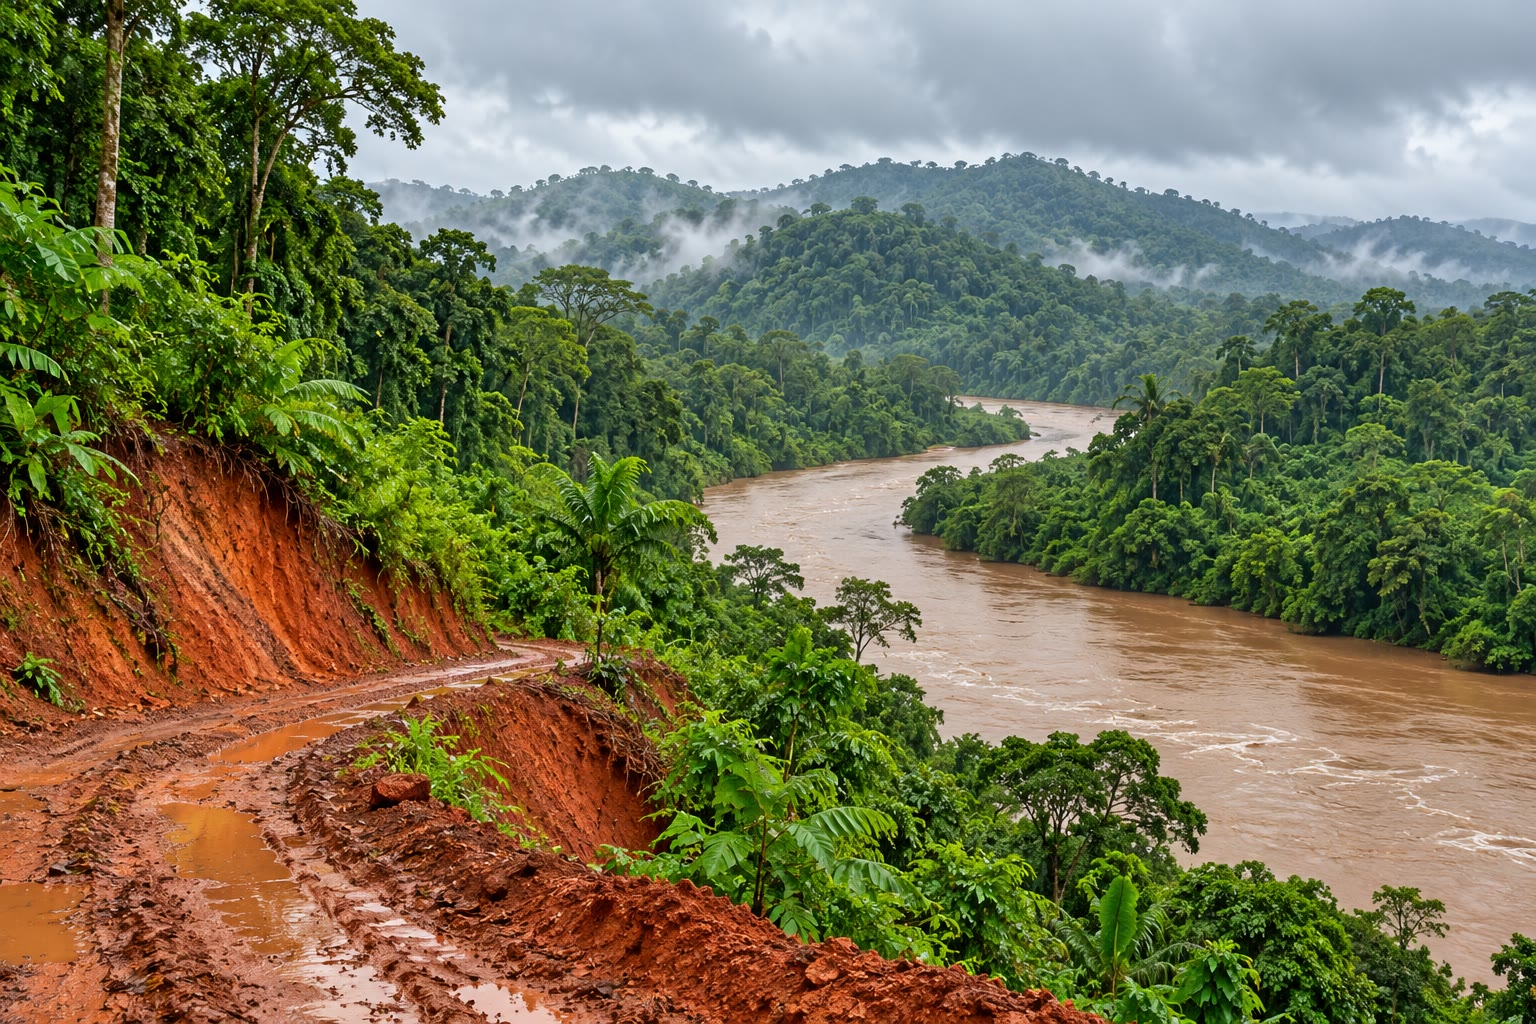
\includegraphics[width=0.66\linewidth]{images/book4/ai/b2-tropical-weathering.jpg}
\par\smallskip{\small Là où le thermostat travaille le plus~: une plaine chaude et humide, où la pluie tombe sur un
sol rouge profondément altéré et où la rivière porte les produits de l'altération jusqu'à la mer
(Illustration générée par IA.)}
\end{omfigure}

\section*{Exercices}\label{sec:b2:deep-time-climate:exercises}

Données des exercices, sauf indication contraire~: carbone préindustriel de l'air
\qty{591}{PgC} (\qty{278}{ppm})~; $\qty{1}{Tmol}$ de carbone $= \qty{0.012011}{PgC}$~;
altération des silicates $W_0 = \qty{0.138}{PgC.an^{-1}}$~; part aérienne d'un excès après l'océan et les carbonates $f = 0.08$~;
sensibilité de l'altération $k_T = \qty{0.09}{K^{-1}}$~; sensibilité climatique $S =
\qty{3}{K}$~; forçage d'un doublement du dioxyde de carbone \qty{3.93}{W.m^{-2}}~; $R =
\qty{8.314}{J.mol^{-1}.K^{-1}}$.
% ledger: ar6ch5:fig512, ipcc:erf-2xco2, derry24:fluxes, colbourn13:timescale, colbourn13:weathering, ipcc:ecs

\begin{exercise}[$\star$]\label{exo:b2:deep-time-climate:1}
Avant l'ère industrielle, l'océan contenait \qty{900}{PgC} dans sa couche de surface, \num{37100} dans ses eaux
intermédiaires et profondes, 700 de carbone organique dissous et 3 dans ses organismes vivants.
(a) Quelle quantité de carbone contenait l'océan, et combien de fois celle de l'atmosphère~? (b) Convertir les
\qty{3.5e6}{Tmol} des réservoirs de surface en pétagrammes de carbone. (c) Quelle part s'en trouve dans
l'air~?
\end{exercise}

\begin{exercise}[$\star$]\label{exo:b2:deep-time-climate:2}
Utiliser les flux de la figure du \omterm{def:b2:deep-time-climate:carbon-cycle}{cycle long du carbone}, en prenant le dégazage métamorphique égal à
\qty{3}{Tmol.an^{-1}}. (a) Additionner les entrées dans les réservoirs de surface et les sorties.
(b) Quelle part des entrées fournissent les volcans, les rifts et le \omterm{def:b2:metamorphic-facies:metamorphism}{métamorphisme}~? (c) Trouver le temps de
séjour du carbone dans les réservoirs de surface, à partir des sorties.
\end{exercise}

\begin{exercise}[$\star$]\label{exo:b2:deep-time-climate:3}
(a) Écrire l'altération de la forstérite, \ce{Mg2SiO4}, par le dioxyde de carbone et l'eau en ions magnésium et
bicarbonate et silice dissoute, \ce{SiO2}, et l'équilibrer. (b) Le magnésium est déposé plus tard sous forme de
carbonate. Écrire la réaction nette. (c) Quelle masse de forstérite doit être altérée pour retirer \qty{1}{PgC} définitivement~?
($M(\ce{Mg2SiO4}) = \qty{140.7}{g.mol^{-1}}$.)
\end{exercise}

\begin{exercise}[$\star$]\label{exo:b2:deep-time-climate:4}
Classer par ordre d'âge, avec leurs dates, et dire pour chacun si la Terre était dans un état de serre ou
un état glaciaire~: l'Optimum climatique de l'Éocène inférieur~; la glaciation hirnantienne~; le début de la
calotte antarctique~; le Turonien~; la plus grande extension de glace du Paléozoïque tardif~; les grandes avancées
des calottes nord~; le PETM.
\end{exercise}

\begin{exercise}[$\star\star$]\label{exo:b2:deep-time-climate:5}
(a) Vérifier qu'une énergie d'activation de \qty{63}{kJ.mol^{-1}} à \qty{288}{K} donne $k_T =
\qty{0.09}{K^{-1}}$. (b) Trouver $k_T$ pour la valeur de terrain \qty{74}{kJ.mol^{-1}}. (c) Avec chacune, trouver le
réchauffement stationnaire lorsque le dégazage augmente de \qty{20}{\percent}. (d) Pourquoi la sensibilité climatique
n'entre-t-elle pas dans (c)~?
\end{exercise}

\begin{exercise}[$\star\star$]\label{exo:b2:deep-time-climate:6}
Comparer le facteur d'Arrhenius exact $\exp[-(E_{\text a}/R)(1/T - 1/T_0)]$ avec $e^{k_T(T -
T_0)}$, $k_T = E_{\text a}/(RT_0^2)$, pour $E_{\text a} = \qty{63}{kJ.mol^{-1}}$ et $T_0 =
\qty{288}{K}$~: (a) à $T = \qty{293}{K}$~; (b) à $T = \qty{318}{K}$. (c) Montrer que le rapport de l'approximation au
facteur exact vaut $\exp[E_{\text a}x^2/(RT_0^2(T_0 + x))]$, avec $x = T - T_0$, et trouver le réchauffement
auquel il atteint 1.1.
\end{exercise}

\begin{exercise}[$\star\star$]\label{exo:b2:deep-time-climate:7}
La compilation lissée donne \qty{1444}{ppm} de dioxyde de carbone à \qty{419.5}{Ma} et \qty{276}{ppm} à la fin de
son enregistrement. (a) Trouver le forçage de cette baisse. (b) Le comparer aux \qty{9}{W.m^{-2}} du Soleil qui se renforce.
(c) Trouver le taux moyen de baisse, en ppm par million d'années, et le comparer aux \qty{3.4}{ppm} de la tendance ajustée.
Pourquoi peuvent-ils différer~?
\end{exercise}
% ledger: data:b4-foster2017, foster17:co2

\begin{exercise}[$\star\star$]\label{exo:b2:deep-time-climate:8}
(a) Répartir \num{3000} et \qty{7000}{PgC} sur 3 et sur \qty{20}{ka}~: quelle plage de vitesses de rejet
en découle~? Comparer avec les 0.3 à \qty{1.5}{PgC.an^{-1}} cités par le GIEC. (b) Les émissions humaines étaient
d'environ \qty{35}{Gt} de dioxyde de carbone en 2010. Convertir en carbone et comparer. (c) Le dioxyde de carbone
est passé de 900 à \qty{2000}{ppm}. Trouver le forçage et le réchauffement d'équilibre avec $S =
\qty{3}{K}$, et comparer avec les \qty{5}{\celsius} de réchauffement par rapport au climat d'avant le PETM.
\end{exercise}
% ledger: ar6ch5:petm-release, usgs:volcanic-co2, ar6ch5:petm

\begin{exercise}[$\star\star$]\label{exo:b2:deep-time-climate:9}
La montée d'une chaîne de montagnes multiplie la capacité d'altération $W_0$ de la Terre par 1.2, à dégazage
constant. (a) Trouver le nouveau changement de température stationnaire. (b) Trouver le nouveau dioxyde de carbone
stationnaire, à partir de \qty{278}{ppm}. (c) Le taux d'altération des silicates, dans le nouvel état stationnaire,
diffère-t-il de l'ancien~? Expliquer.
\end{exercise}

\begin{exercise}[$\star\star\star$]\label{exo:b2:deep-time-climate:10}
(a) Trouver le temps caractéristique de décroissance du thermostat avec le facteur de ruissellement,
$k = 0.09 + 0.65\times0.045$. (b) Sur des millions d'années, les calottes et la végétation réagissent aussi~; avec une
sensibilité du système Terre de \qty{8}{K} par doublement au lieu de $S$, trouver $\tau$ avec $k_T$. (c) Dans quel sens
les deux changements poussent-ils le thermostat, et quelle incertitude, $E_{\text a}$ ou $S$, compte le plus~?
\end{exercise}

\begin{exercise}[$\star\star\star$]\label{exo:b2:deep-time-climate:11}
Un rejet de \qty{5000}{PgC} (après l'océan et les carbonates). (a) Trouver le dioxyde de carbone de
l'air, en ppm, et le réchauffement. (b) Trouver le taux net initial d'élimination $W - W_0$, et le temps que
mettrait l'impulsion à disparaître à ce rythme. (c) Trouver le temps linéarisé pour éliminer \qty{90}{\percent}
de l'excès. (d) Le modèle, intégré sans linéarisation, prend \qty{340}{ka}. Pourquoi plus long~?
\end{exercise}

\begin{exercise}[$\star\star\star$]\label{exo:b2:deep-time-climate:12}
(a) Linéariser le modèle autour d'un état stationnaire où le dégazage vaut $V$ et $C = C^*$, et montrer que le
temps caractéristique est $\tau' = A_0 (C^*/C_0)\ln 2/(f k S V)$. (b) Le calculer pour l'état stationnaire d'une
hausse de \qty{20}{\percent} du dégazage. (c) Le thermostat est-il plus rapide ou plus lent dans un monde riche en
dioxyde de carbone, et pourquoi~?
\end{exercise}

\begin{problem}[{Problème du week-end --- Combien de temps met le thermostat~?}]\label{pb:b2:deep-time-climate:1}
Ce problème construit le temps caractéristique du thermostat à partir de flux mesurés. Utiliser les données des
exercices~; dégazage aux dorsales, aux \omterm{def:b2:oceanic-islands:stages}{îles océaniques}, aux arcs et aux rifts \num{1.3}, \num{1.3}, 4.5 et
\qty{4.2}{Tmol.an^{-1}}~; altération des silicates de 11 à \qty{12}{Tmol.an^{-1}}~; énergie d'activation
\qty{63}{kJ.mol^{-1}} à $T_0 = \qty{288}{K}$~; masse de l'atmosphère \qty{5.1e18}{kg}, masse molaire moyenne
de l'air \qty{28.97}{g.mol^{-1}}. Arrondir à trois chiffres significatifs.

\noindent\textbf{Partie I --- Bilan.}
\begin{enumerate}
  \item Additionner le dégazage volcanique et celui des rifts, en \unit{Tmol.an^{-1}} et en \unit{PgC.an^{-1}}.
  \item Prendre $W_0$ au milieu de son intervalle~; le convertir en \unit{PgC.an^{-1}}.
  \item Comparer les deux. Qu'indique la comparaison sur le \omterm{def:b2:deep-time-climate:carbon-cycle}{cycle long du carbone}~?
  \item Combien de moles d'air contient l'atmosphère~? Combien de moles de carbone représentent \qty{591}{PgC},
        et quel \omterm{def:b2:atmospheric-thermodynamics:moist-air}{rapport de mélange} cela donne-t-il~?
  \item Sans aucune altération, combien de temps mettrait le dégazage de la question 1 pour ajouter
        \qty{591}{PgC} aux réservoirs de surface~?
  \item Si une fraction $f = 0.08$ en restait dans l'air, de quel facteur le dioxyde de carbone de l'air
        augmenterait-il~?
\end{enumerate}

\noindent\textbf{Partie II --- Linéarisation.}
\begin{enumerate}[resume]
  \item Trouver $k_T$ à partir de l'énergie d'activation, et vérifier qu'il s'arrondit à la
        valeur \qty{0.09}{K^{-1}} utilisée plus bas.
  \item De quel facteur l'altération croît-elle pour un réchauffement de \qty{1}{K}~?
  \item Écrire le réchauffement $\Delta T$ pour un excès $M$, et sa dérivée en $M = 0$, en
        \unit{K.PgC^{-1}}.
  \item Trouver la dérivée de $W$ par rapport à $M$ en $M = 0$, en \unit{an^{-1}}.
  \item Montrer que son inverse est le temps caractéristique $\tau$ de la
        \cref{prop:b2:deep-time-climate:thermostat}.
  \item Lesquels parmi $f$, $k$, $S$ et $W_0$ rendent le thermostat plus rapide lorsqu'ils augmentent~?
\end{enumerate}

\noindent\textbf{Partie III --- Le temps caractéristique.}
\begin{enumerate}[resume]
  \item Évaluer $\tau$.
  \item L'évaluer avec le facteur de ruissellement, $k = \qty{0.119}{K^{-1}}$.
  \item L'évaluer avec $k_T$ et une énergie d'activation de \qty{74}{kJ.mol^{-1}}.
  \item Comparer ces valeurs aux \qty{200}{ka} à \qty{1}{Ma} des modèles à océan explicite.
  \item Combien de temps caractéristiques de décroissance tiennent dans les \qty{50}{Ma} de baisse du dioxyde de
        carbone du Cénozoïque~? Que dit cela de l'état du cycle du carbone pendant la baisse~?
  \item À \qty{16}{ppm} par million d'années, de combien le dioxyde de carbone varie-t-il en un $\tau$~?
\end{enumerate}

\noindent\textbf{Partie IV --- Un rejet de la taille du PETM.}
\begin{enumerate}[resume]
  \item \qty{5000}{PgC} sont libérés~; combien restent dans l'air une fois que l'océan et les carbonates
        ont agi, et quel est le dioxyde de carbone en ppm~?
  \item Trouver le réchauffement à cet instant.
  \item De combien le taux d'altération augmente-t-il, en \unit{PgC.an^{-1}} et en pourcentage~?
  \item Avec la loi linéarisée, combien de temps faut-il pour que \qty{90}{\percent} de l'excès disparaissent~?
  \item Le carbonate du PETM s'est rétabli sur environ \qty{100}{ka}. Donner deux raisons pour lesquelles la
        Terre réelle a pu être plus rapide que ce modèle.
  \item En résumé, quel est le temps caractéristique de décroissance du \omterm{def:b2:deep-time-climate:thermostat}{thermostat de l'altération des silicates} dans ce modèle~?
\end{enumerate}
\end{problem}
% ledger: derry24:fluxes, colbourn13:weathering, colbourn13:timescale, ar6ch5:fig512, ar6ch5:petm, ar6ch5:cenozoic-co2, ipcc:ecs, earth:Matm, earth:Mmol
